 %-*- root: ../InvestigacionOperativa.tex -*-

\section{Hoja 1}

\begin{problem}[1]

Una empresa de reciclaje usa papel y tela desechados para fabricar dos tipos distintos de papel reciclado.
Cada tanda de papel reciclado de clase A requiere 20 kg de tela y 180 kg de papel y produce un beneficio de 500 euros, mientras que cada tanda de papel reciclado de clase B requiere 10 kg de tela y 150 kg de papel y produce un beneficio de 250 euros. 
La compañía dispone de 100 kg de tela y 660 kg de papel. ¿Cuántas tandas debe fabricar de cada tipo?

\solution

\begin{center}
\begin{tabular}{c|ccc}
& A & B & Disp. \\\hline
Tela & 20 & 10 & 100\\
Papel & 180 & 150 & 660\\
Beneficio & 500 & 250 & 
\end{tabular}
\end{center}

Variables $x = $ calidad de A e $y = $ calidad de B.

\begin{ioprob}
\goal{$\max 500x_1 + 250 x_2$}
\restrictions{$20x_1 + 10x_2 \leq 100$}{$180x_1 + 160x_2 \leq 660$}{$x_i \geq 0$}{}{}{}
\end{ioprob}

Vamos a resolverlo gráficamente en la figura \ref{ej:1.1.a}. Vamos a reprensentar el conjunto del plano que cumple las 3 restricciones.


\begin{figure}[hbtp]
\centering
\begin{tikzpicture}[scale=0.6]
\draw[thick,->] (-1,0) -- (10,0) node[anchor=west] {$x$};
\draw[thick,->] (0,-1) -- (0,10) node[anchor=east] {$y$};
\draw[thick,-] (5,0) -- node[anchor=north west] {\text{ }$20x + 10 y = 100$} (0,10);
\draw[thick,-] (3.8,0) -- node[anchor=west] {$180x + 150y = 660$} (0,4);
\filldraw[fill=blue!40!white, pattern=north west lines, pattern color=blue] (0,0) -- (0,4) -- (3.8,0);
\draw[thick,-,color=red] (2,-2) -- (-1,4);
\draw (3.8,0) node[anchor=north]  {$(3.8,0)$};
\draw [shorten >= 3cm, shorten <= -4cm,color=red,thick] (3.8,0) -- +($(2,-2)-(-1,4)$);
\end{tikzpicture}
\label{ej:1.1.a}
\caption{Representamos las 2 rectas fronteras y el vector gradiente de la función objetivo.}
\end{figure}


La idea es mover la recta roja en su dirección perpendicular todo lo que podamos. En este caso, no podremos alejarnos más que el punto que del punto $(3.8,0)$, con lo que será el óptimo.

\end{problem}


\begin{problem}[2]

La empresa Animales Salvajes S.A. cría faisanes y perdices para repoblar el bosque y dispone de sitio para criar 100 pájaros durante la temporada.
Criar un faisán cuesta 20 euros y criar una perdiz cuesta 30 euros. 
La fundación Vida Animal paga a Animales Salvajes S.A. por los pájaros de forma que se obtiene un beneficio de 14 euros por cada faisán y 16 euros por cada perdiz. 
La empresa dispone de 2400 euros para cubrir costes. ¿Cuántas perdices y cuántos faisanes debe criar?


\solution 


\begin{center}
\begin{tabular}{c|cccc}
&Faisán & Perdiz & Disp. & \# pájaros \\\hline
Coste&20&30&2400&100\\
Beneficio&14&16&
\end{tabular}
\end{center}

Las variables utilizadas son $x$ para Faisán e $y$ para Perdiz.

El problema a resolver sería:

\begin{ioprob}
\goal{$\max 14x + 16y$}
\restrictions{$x+y\leq 100$}{$20x + 30y \leq 2400$}{$x,y > 0$}{}{}{}
\end{ioprob}

En la figura \ref{ej:1.2.a} encontramos la solución gráfica del problema. Vemos que la solución es la intersección de las rectas, así que calculamos la intersección: 
\[
\left.
	\begin{array}{cc}
		x+y = 100 \\ 
		20x+30y = 2400
	\end{array}
\right\} 
\to (x,y) = (40,60)
\]

\begin{figure}[h]
\centering
\begin{tikzpicture}[scale=0.6]
\draw[thick,->] (-1,0) -- (12.5,0) node[anchor=west] {$x$};
\draw[thick,->] (0,-1) -- (0,12.5) node[anchor=east] {$y$};
\draw[thick,-] (10,0) --  node[anchor=west] {$x+y=100$} (0,10);
\draw[thick,-] (8,0) -- (0,12) node[anchor=west] {$20x + 30y = 2400$};
\filldraw[fill=blue!40!white, pattern=north west lines, pattern color=blue] (0,0) -- (0,10) -- (4,6) -- (8,0);
\draw[thick,-,color=red] (3.5,0) -- (0,4);
%\draw[thick,-,color=green] (9,0) -- (0,11);
\draw [shorten <= -4cm,shorten >= -2cm, ,color=green,thick] (4,6) -- +($(3.5,0)-(0,4)$);
\end{tikzpicture}
\label{ej:1.2.a}
\caption{Representamos las 2 rectas fronteras y el vector gradiente de la función objetivo. En rojo la dirección del gradiente y en verde la solución óptima.}
\end{figure}





\end{problem}


\begin{problem}[3]

La siguiente tabla da el porcentaje de proteínas, grasas y carbohidratos, para cinco alimentos
básicos, A, B, C, D y E :


Los precios por 100 g de estos alimentos (dados en el mismo orden de la tabla) son 5, 17, 37, 10,
15. Si una persona necesita consumir como mínimo 75 gramos de proteínas, 90 de grasas y 300 de
hidratos de carbono, plantea el problema de minimización para calcular la dieta alimenticia de mínimo coste.
\solution


\end{problem}


\begin{problem}[9]

Una propiedad conocida de la mediana de un conjunto de datos $y_i$ es que minimiza en $\theta$ el valor de $\sum y_i-\theta$. Plantea el problema de optimización como un problema lineal en forma estándar.
\solution

Queremos minimizar 
\[\sum_{i=1}^n |y_i - \theta|\]

El procedimiento habitual podría ser derivar e igualar a 0, pero en este caso no podemos ir por ese camino, ya que no es derivable.
Vamos a ver que la solución es la mediana y vamos a demostrarlo de 2 maneras distintas. 
Primero, formalmente y después, planteándolo como un problema de optimización lineal.

\begin{proof}

Tomando una muestra de tamaño 2 y un punto interior de $\theta$ el objetivo a minimizar es:
\[\sum |y_i - \theta| = \theta - y_{(1)} + y_{(2)}-\theta = y_{(2)} - y_{(1)}\]
es decir, la longitud del intervalo.

Vamos a tomar una muestra de tamaño $n$. 
En esa muestra,tTomamos una serie de intervalos contenidos de la siguiente manera:

\[ [y_{(1)},y_{(n)}] \supset  [y_{(2)},y_{(n-1)}] \supset [y_{(3)},y_{(n-2)}] \supset ... \supset [y_{(m)},y_{(n-m+1)}]\]

Donde \[m=\left\{ \begin{array}{cc} \frac{n}{2} & n\text{ par}\\ ?? & n\text{ impar} \end{array}\right.\]
Este es un razonamiento casi geométrico de porque la mediana minimiza.
\end{proof}


Ahora, vamos a contestar al enunciado, planteándolo como un problema de regresión.

Definimos $x_i \equiv y_i - \theta = x_i^+ - x_i^-$ donde $x_i^+ = \max\{x_i,0\}$ y $x_i^- = \max\{-x_i,0\}$

De esta manera, $\abs{x_i} = x_i^+ + x_i^-$. Con este truco, hemos conseguido modificar la función objetivo, que de esta manera es una función lineal.

Nuestra función objetivo es:

\[\min \sum_{i=1}^n x_1^+ + x_i^-\]

Y el precio a pagar, es que necesitamos incluir una restricciones, con lo que:


\begin{ioprob}
\goal{\[\min \sum_{i=1}^n x_1^+ + x_i^-\]}
\restrictions{$y_i = x_i^+ - x_i^- + \theta^+ + \theta^-$, $i=1,...,n$}{$x_i^+ \geq 0$}{$x_i^- \geq 0$}{$\theta_i^+ \geq 0$}{$\theta_i^+ \geq 0$}{}
\end{ioprob}


Vamos a escribirlo matricialmente.
Las \textbf{variables de decisión} son $(x_1^+,...,x_n^+,x_1^-,...,x_n^-,\theta^+,\theta^-$. 

\[c = (\underbrace{1,...,1}_{n},\underbrace{1,...,1}_{n},0,0)\]
\[b = (y_1,...,y_n) \]
\[A = \left( I | -I | 1_n | -1_n\right)\to \begin{array}{c}1_n = \begin{pmatrix}1\\1\\\vdots\\1\end{pmatrix}\\ I = \text{ identidad} \end{array}\]




\obs{}
¿Qué utilidad puede tener esto?
Al tomar un modelo de regresión (una recta que pase por una nube de puntos) se suele tomar el criterio de "mínimos cuadrados", que es minimizar $\sum y_i-(β_0+β_1x_i)$ (siendo $β_0+β_1x$ el modelo de regresión). 
Podríamos plantear un modelo de regresión con otro criterio, por ejemplo, el de minimizar el valor absoluto.




\end{problem}



\section{Hoja 3}
\begin{problem}[1]
Sea $S\subset \real^n$. Dado $ε\geq 0$, la dilatacińo de $S$ se define como \[S_ε = \{x:d(x,S)\leq ε\}\] donde \[d(x,S) = \inf_{y\in S}{\norm{x-y}}\]

La erosión de $S$ se define como 
\[S_{-ε} = \{x:B(x,ε) \subset S \} \]

Demuestra que si $S$ es convexo, entonces tanto $S_{ε}$ como $S_{-ε}$ son conjuntos convexos

\solution
\doneby{Uceda}

\end{problem}


\begin{problem}[2]
Sean $x_0,...,x_k \in \real^n$. Considera los puntos que están más cerca de $x_0$ que de otro de los puntos $x_i$, es decir,

\[V = \{x\in\real^n : \norm{x-x_0}\leq \norm{x-x_i}\;,i=1,...,k\}\]

El conjunto $V$ se llama \textbf{región de Voronoi} de $x_0$ respecto de $x_1,...,x_k$

\ppart Demuestra que $V$ es un poliedro. Determina la matriz $A$ y un vector $b$ tales que $V = \{x\in\real^n Ax\leq b\}$

\ppart Recíprocamente, dado un poliedro $P$ con interior no vacío, determina $x_0,...,x_k$ de manera que $P$ sea la región de Voronoi de $x_0$ respecto de $x_1,...,x_k$.

\solution
\todoby{Uceda}
\end{problem}


\begin{problem}[3]

Sea $S\subset \real^n$ un conjunto convexo no vacío y sean $λ_1 > 0$ y $λ_2 > 0$.

\ppart Demuestra que $(λ_1 + λ_2)S = λ_1S + λ_2S$

\ppart Determina razonadamente si es cierta o no la propiedad del apartado anterior cuando el conjunto $S$ no es convexo.

\solution

\end{problem}

\begin{problem}[4]
Sea $S\subset \real^n$ un conjunto cerrado tal que si $x_1,x_2\in S$, entonces $(x_1 + x_2)/2 \in S$. Demuestra que $S$ es convexo.

\solution

El punto medio de un segmento es el límite de una sucesión de puntos dentro del segmento. Vamos a escribirlo formalmente.


Sean $x,y\in S$ y queremos ver si \[λx + (1-λ)y \in S\; ∀λ\in(0,1)\]

Una manera de formalizar esto es escribir $λ$ como:

\[λ = \sum_{i=1}^{∞} \frac{i_1}{2^i}\;\; c_i\in {0,1}\]

Y llamamos $λ_k = \sum^k$. De esta manera,

\[ λ_1x + (1-λ_1)y = \left\{ \begin{array}{cc} \frac{x+y}{2}\in S & λ_1 = \rfrac{1}{2}\\ y\in S & λ_1 = 0 \end{array} \right. \]

Por inducción, \[λ_kx + (1-λ_k) y \in S \implies λ_{k+1}x + (1-λ_{k+1})y \in S\]

Se deja como ejercicio del ejercicio escribir por inducción esta prueba.


\end{problem}

\begin{problem}[5]

Sea $X_1,...,X_n$ una muestra de $n$ vectores independientes e idénticamente distribuidos,
con distribución uniforme en el cuadrado unidad $S = [0, 1]^2$. 
Consideramos la variable aleatoria N n correspondiente al número de vértices del cierre convexo de $X_1,...,X_n$.

\ppart Escribe una función en R que dos argumentos n y B, y que dé como resultado un vector con B realizaciones de la variable N n .
\ppart Genera $B = 10000$ realizaciones de la v.a. $N_n$ para $n = 100$. Calcula la media y la
desviación típica de los valores obtenidos y representa el correspondiente histograma.
¿A qué distribución se parece el histograma obtenido?

\solution

\end{problem}


\begin{problem}[6]
Demuestra que si $S ⊂ \real^n$ es un conjunto convexo, entonces $\text{int}(S) = \gor{S}$ también son
conjuntos convexos.

\solution

Si $x\in \gor{S}$ e $y\in\text{int}(S)$, entonces $λx + (1-λ)y \in \text{int}(S)$ (es un lema que ya hemos visto).

Utilizando este lema, Tenemos que provar que $S$ convexo $\implies \gor{S}$ convexo.

\[x,y \in \gor{S}, λ\in(0,1) \implies ∃\{x_k\},\{y_k\} \tlq x_k \to x \wedge y_k \to y\]

Por otro lado, tenemos \[λx + (1-λ)y \in \gor{S}\; ¿λ∈(0,1)?\].

Vamos a tomar la combinación convexa con $λ$ y con las sucesiones, es decir:
\[λx_k + (1-λ)y_k \to λx + (1-λ)y \in \gor{S}\]

\end{problem}

\begin{problem}[7]
Sea $S\subset\real^n$ un conjunto convexo con $\text{int}(S)≠\emptyset$. Demuestra $\gor{S}=\gor{\text{int}(S)}$.

\solution

Una de las 2 inclusiones es obvia y la otra no. Vamos a ver la complicada:

$\gor{S} \subset \text{int}(\gor{S})$:

Utilizando un argumento parecido al anterior, utilizamos $λx_0 + (1-λ)x \in\text{int}({S})$ y haciendo tender $λ\to 0$ obtenemos $x\in \text{int}(\gor{S})$

\spart $\text{int}(\gor{S}) = \text{int}({S})$

Si es vacío, los 2 son vacíos. En caso de no ser vacío, tenemos que probar que:

\[x\in\text{int}(\gor{S}) \implies x \in \text{int}(S)\]

Consideramos el segmento que va de $y$ a $x$ y prolongamos un poco el segmento, hasta un punto $z$ que esté en el cierre, en $\text{int}(\gor{S})$. De esta manera, $x$ queda en un segmento que une un punto del interior ($y$) con uno del cierre $(z)$, con lo que $x$ está en el interior.
\end{problem}


\begin{problem}[8]
Da un ejemplo para probar que el cierre convexo, $\convx{S}$, de un conjunto cerrado no
es necesariamente cerrado. Utiliza el teorema de Caratheodory para probar que si $S$ es
compacto, entonces $\convx{S}$ es compacto.

\solution

\[S_1 = \{(x_1,x_2) \in \real^2: x_1 \geq 0 \; x_2 = 0\}\]
\[S_2 = \{(x_1,x_2) \in \real^2: x_1 = 0\; 0\leq x_2\leq 1\}\]

\begin{figure}[hbtp]
\centering
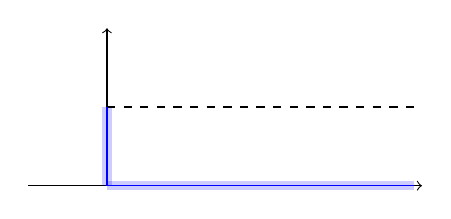
\begin{tikzpicture}
\draw[->] (-1,0) -- (4,0);
\draw[->] (0,1) -- (0,2);
\draw[color=blue] (0,1) -- (0,0);
\fill[opacity = 0.2, blue] (-0.4ex,0) -- (-0.4ex,1) -- (0.4ex,1) -- (0.4ex,0) -- cycle;
\fill[opacity = 0.2, blue] (0,-0.4ex) -- (3.9, -0.4ex) -- (3.9, 0.4ex) -- (0,0.4ex) -- cycle;
\draw[color=blue] (0,0) -- (3.9,0);
\draw[dashed] (0,1) -- (4,1);
\end{tikzpicture}
\caption{Representación gráfica de la unión de $S_1$ y $S_2$}
\end{figure}

\spart

\[\convx{S} = \{x = \sum^{n+1}λ_ix_i\;λ_i \geq 0, \sum λ_i = 1\; x_i\in S\}\]

Tomando \[k = \{(λ_1,λ_2,...,λ_{n+1},x_1,...,x_{n+1}) \;λ_i \geq 0, \sum λ_i = 1\; x_i\in S\}\]

Y construimos: $\appl{f}{k}{\convx{S}}$ tal que $f(λ_1,λ_2,...,λ_{n+1},x_1,...,x_{n+1}) = \sum^{n+1}λ_ix_i$ y esta función es continua.

Tenemos $k$ compacto (por ser $S$ compacto) y que  $f(k) =\convx{S}$, siendo $f$ continua. Entonces, $\convx{S}$ es compacto (por ser imagen continua de un compacto).

\end{problem}

\begin{problem}[9]

Encuentra un ejemplo que muestre que la implicación

\[S_1,S_2 \text{ convexos cerrados} \implies S_1+S_2\text{ es cerrado}\]

no es cierta en general. Prueba que esta implicación es cierta cuando al menos uno de los 2 conjuntos $S_1$ o $S_2$ se supone compacto.

\solution

\[S_1 = \{ (x_1,x_2) \in \real^2\tq\; x_2\geq \rfrac{1}{x_1} \;x_1 > 0\}\]
\[S_2 = \{(x_1,0) \in \real^2\tq x_1\in\real\}\]

Vamos a construir $S_1 + S_2$


\begin{figure}[hbtp]
\centering
\begin{tikzpicture}
\draw[->] (-1,0) -- (4,0);
\draw[->] (0,-1) -- (0,4);
\fill[opacity = 0.5,black,pattern=north east lines] (4,4) -- plot[variable=\t,samples=25,domain=0.25:4] (\t,1/\t);
\end{tikzpicture}
\caption{Representación gráfica de la suma de $S_1$ y $S_2$}
\end{figure}


\[S_1 + S_2  = \{(x_1,x_2)\tlq x_2>0\}\]

\[(0,0) = \lim (\underbrace{x_k}_{\in S_1} + \underbrace{y_k}_{S_2})\]

Para que sea la suma sea cerrada, necesitaríamos $\{y_k\},\{x_k\} \to (0,0)$ y en este caso no es así. Vamos a ver que con que uno de los 2 conjuntos sea acotado, la suma ya es acotada.

\begin{prop}

$S_1,S_2$ convexos y cerrados, con $S_1$ acotado.

Tomamos $x_k + y_k \in S_1 + S_2$ y tenemos $\lim(x_k + y_k) = z$.

Entonces,
\[z\in S_1 + S_2\]
\end{prop}
\begin{proof}
Existe una subsucesión convergente $\{x_{k_i}\}$de $\{x_k\}$, por ser $S_1$ compacto.
Sea $\gor{x} = \lim x_{k_i}$, con $\gor{x}\in S_1$.

La correspondiente subsucesión de $y_k$ también converge (ya que sino la suma no puede converger)

\end{proof}

\end{problem}

\begin{problem}[10]

$S$ convexo es la intersección de todos los subespacios cerrados que lo contienen.

Formalmente:

\[S = \bigcap_{\begin{array}{c}S\subset H_i\\H_i\text{ compacto}\end{array}} H_i\]

\solution

$S\in \bigcap$ es trivial. 

\[\left.\begin{array}{c} x\in\bigcap H_i\\x\not\in S \end{array}\right\} \implies \exists p≠0, α\in\real p^ty\leq α ∀y\in S p^t x >α\]


\end{problem}

\begin{problem}[11]

Sean $S_1,S_2$ dos conjuntos convexos no vacíos de $\real^n$ tales que $S_1\cap S_2 = \emptyset$. 
Demuestra que existe $p ∈ \real^n , p≠0$, tal que

\[\inf\{p^Tx: x\in S_1\} \geq \sup\{p^Tx : x\in S_2\}\]

Si además, los conjuntos son cerrados y uno de ellos es acotado, demostrar que existe $\rho \in \real^n,\rho ≠ 0, ε > 0$ tales que 

\[\inf\{p^Tx: x\in S_1\} \geq ε + \sup\{p^Tx : x\in S_2\}\]

\textit{Sugerencia: Para la primera parte, considera $S = \{x_1 - x_2 : x_1 \in S_1, x_2 \in S_2\}$ y aplica algún teorema de separación}

\solution


\[ S = \{x_1-x_2 \tq x_1\in S_1, x_2\in S\]

Es convexo, y tenemos $S_1\cap S_2 = 0 \implies 0\not\in S$.

Por ser $\gor{S}$ cerrado y convexo, tenemos 2 posibilidades $0\in S$ o $0\not\in S$:
\[0\not\in \gor{S}\implies \exists p≠0, \exists α\in ℝ p^tx\geq α>0 ∀x\in S\]

\[
\implies p^tx_1 \geq α + p^tx_2 ∀x_i\in S_i
\]


Si por el contrario:

\[
0\in \gor{S} - S \implies 0 \in \partial S \implies \exists p≠0, p^tx\geq 0, ∀x\in S
\]

Eso último se debe a $p^tx_1 ≥ p^tx_2, ∀x_i\in S_i$



\end{problem}

\begin{problem}[12]

\solution

\begin{defn}[Función\IS soporte]
\[S_c(p) = \sup\{p^tx\;:x\in C\}\]
La utilidad de la función soporte es poder comparar funciones en vez de trabajar con conjuntos. Esto está muy bien porque en general es más fácil trabajar con funciones que con conjuntos sobretodo en temas de convergencia.
\end{defn}



Queremos probar que:

\[C = D \dimplies S_C(p) = S_D(p)\]

$\implies)$: Trivial

$\impliedby)$: Supongamos que existe $\gor{x}\in D \tlq \gor{x}\notin C$. De esta manera, podemos aplicar un teorema de separación, es decir:

\[∃p≠0 \tlq p^tx≤α ∀x∃C \implies S_C(p) ≤α \wedge S_D(p) > α \]


\end{problem}

\begin{problem}[13]
Demuestra que si $x$ es una solución factible básica de $S = \{x : Ax = b, x ≥ 0\}$, entonces
es un punto extremo de S.

\solution

$x$ es una solución factible básica si al elegir una base, tenemos: \[x = \begin{pmatrix}B^{-1}b\\0\end{pmatrix} \equiv \begin{pmatrix}\gor{b}\\0\end{pmatrix}\]

Vamos a escribir $x$ como combinación convexa de puntos y ver que esos puntos son iguales a $x$, es decir:

\[\begin{pmatrix}B^{-1}b\\0\end{pmatrix} = λx_1 + (1-λ)x_2 = λ\begin{pmatrix}X_{1B}\\X_{1N}\end{pmatrix} + (1-λ)\begin{pmatrix}X_{2B}\\X_{2N}\end{pmatrix}\]

Como $x_1≥0,x_2≥0 \implies X_{1N} = X_{1B} = 0$. Entonces, tenemos para $i=1,2$:

\[x_i = \begin{pmatrix}X_{iB}\\0\end{pmatrix} \implies Bx_{iB} + N0 = b \implies x_{iB}B^{-1}b = \gor{b}\]


\end{problem}


\begin{problem}[14]
Halla los puntos extremos de los siguientes conjuntos:

\ppart $S = \{(x_1,x_2) \in \real^2 : x_1 + 2x_2 \geq 2, -x_1+x_2 = 4, x_1,x_2\geq 0\}$
\ppart $S = \{(x_1,x_2,x_3) \in \real^3 : x_1 + x_2 + x_3 \leq 10, -x_1+2x_2 = 4, x_1,x_2,x_3\geq 0\}$

\solution

\spart 
\label{ej:ejercicio2.14.a}
Aunque el problema se puede resolver sólo gráficamente, vamos a solucionarlo también algebraicamente.


\begin{figure}[hbtp]
\centering
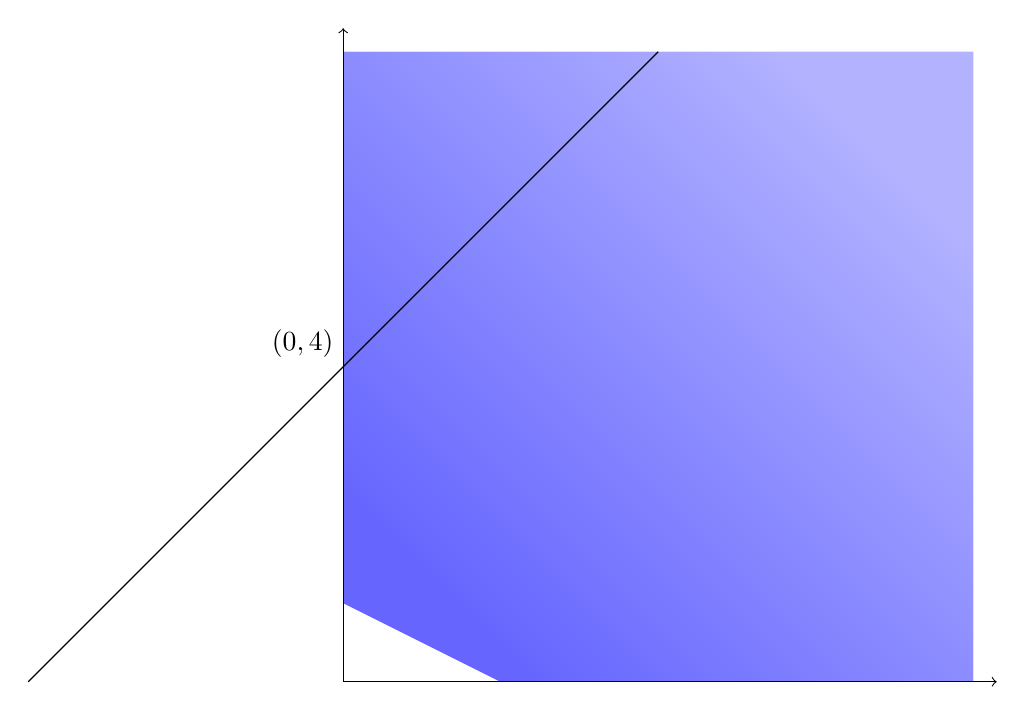
\begin{tikzpicture}
\fill[shading = axis,rectangle, left color=blue!60!white, right color=blue!30!white,shading angle=135,blue!60!white] (0,1) -- (2,0) -- (8,0) -- (8,8) -- (0,8);
\node[anchor=south east] at (0,4) {$(0,4)$};
\draw (-4,0) -- (0,4) -- (4,8);
\draw[->] (0,0) -- (0,8.3);
\draw[->] (0,0) -- (8.3,0);
\end{tikzpicture}
\caption{Solución gráfica del \fref{ej:ejercicio2.14.a}}
\end{figure}

Para resolverlo algebraicamente, tenemos que ir probando con las bases hasta obtener $\gor{b} ≥ 0$. Lo primero que hay que hacer es reconstruir con las variables de holgura, es decir:

\[S = \{(x_1,x_2) \in \real^2 : x_1 + 2x_2 - x_3 = 2, -x_1+x_2 = 4, x_1,x_2,x_3\geq 0\}\]


La solución es:

\[
B = \begin{pmatrix}2&-1\\1&0\end{pmatrix} \implies \gor{b} = \begin{pmatrix}4\\6\end{pmatrix} ≥ \begin{pmatrix}0\\0\end{pmatrix}
\]

\spart 

\todoby{Uceda}

\begin{figure}[hbtp]
\centering
\begin{tikzpicture}
\draw[->] (0,0,0) -- (0,0,4);
\draw[->] (0,0,0) -- (0,4,0);
\draw[->] (0,0,0) -- (4,0,0);
\end{tikzpicture}
\end{figure}
\end{problem}


\section{Hoja 3}

\begin{problem}[1]

Resolver utilizando el algoritmo de simplex el problema:

\begin{ioprob}
\goal{$x_2 - 3x_3 + 2x_5$}
\restrictions{$x_1+3x_2-x_3+2x_5 = 7$}{$-2x_2 + 4x_3 + x_4 = 12$}{$-4x_2 + 3x_3 + 8x_5 + x_6 = 10$}{$x_i \geq 0$}{}
\end{ioprob}

\solution

Vamos a construir la tabla del simplex:


\begin{table}[hbtp]
\centering
\begin{tabular}{c|cccccc}
$c_j$&0&1&-3&0&2&0\\\hline
Variables & $x_1$&$x_2$&$x_3$&$x_4$&$x_5$&$x_6$\\\hline
7&1&3&-1&0&2&0\\
12&0&-2&\textcolor{red}{4}&1&0&0\\
10&0&-4&3&0&8&1\\\hline
$z_j - c_j$ & 0&-1&3&0&-2&0
\end{tabular}
\end{table}

Incluimos la solución final, para terminar el problema en casa. Tras 2 iteraciones obtenemos:


\begin{table}[hbtp]
\centering
\begin{tabular}{c|cccccc}
\hline
4&$\rfrac{2}{5}$&1&0&0.1&0.8&0\\
5&0.2&1&0.3&0.4&0\\
11&1&0&0&-0.5&10&1\\\hline
&-0.2&0&0&-0.8&$-\rfrac{12}{5}$&0
\end{tabular}
\end{table}

Entonces, la solución sería:

\[
\gor{x} = (0,4,5,0,0,11)
\]
\end{problem}

\begin{problem}

\solution
\todoby{Uceda}
\end{problem}

\begin{problem}[3]

\solution

Lo primero es escribir el problema en forma estándar:


\begin{ioprob}
\goal{$\min \sum_{i=1}^3 c_ix_i$}
\restrictions{$x_1-x_2+5x_3 + x_4 = 10$}{$2x_1 - x_2 + x_3 + x_4 = 40$}{$x_i \geq 0$}{}{}
\end{ioprob}

\spart 

Cogemos una base y operamos:

\[B = \begin{pmatrix}1&0\\0&1\end{pmatrix} \to B^{-1}b = b = \begin{pmatrix}10\\40\end{pmatrix}\geq \begin{pmatrix}0\\0\end{pmatrix} \to (0,0,0,10,40)\]

Como $B^{-1}b \geq 0$, $(0,0,0,10,40)$ es un punto extremo.

Tomando por ejemplo:

\[B = \begin{pmatrix}5&0\\3&1\end{pmatrix} \to ... \to (0,0,2,0,34)\]
 
Obtenemos otro punto extremo.

\textbf{Dirección extrema} 

\[
B= 
	\begin{pmatrix}
	1&0\\
	0&1
	\end{pmatrix}\;\; 
a_j = a_2\implies B^{-1}a_2 = 
\begin{pmatrix}
-1\\
-1
\end{pmatrix}\geq 
\begin{pmatrix}
0\\
0
\end{pmatrix} \to d = α
\begin{pmatrix}
0\\
1\\
0\\
\hline 1\\1
\end{pmatrix}\]

\spart

Para cualquier $c_1,c_3$, mientras tomemos $c_2$ negativo no vamos a tener nunca una solución óptima. 

\spart 

Para tener infinitas soluciones óptimas, necesitamos vectores de coeficientes distintos que nos den el mismo valor objetivo.

Podemos tomar $c_1,c_2,c_3$ de tal manera que los 2 puntos extremos que tenemos calculados antes tengan el mismo valor objetivo. De esta manera,  el segmento que une los 2 puntos tiene el mismo valor objetivo. 
\end{problem}


\begin{problem}[4]

Dado un problema de optimización lineal $\min c^\top x$, sujeto a $Ax = b, x ≥ 0$, ¿es posible conseguir un
problema en el que no exista solución óptima finita cambiando únicamente el vector b? Responde a
la misma pregunta para el vector c

\solution

Los teoremas de caracterización nos daban una condición de existencia de solución en caso de cosas en las que no influye $b$, por lo que $b$ no influye y por lo tanto no es posible conseguirlo.

En cuanto al $c$, simplemente con cambiarlo de signo se revienta todo.

\end{problem}
